\documentclass[a4paper,10pt]{article}

\usepackage[ansinew]{inputenc}
\usepackage[spanish]{babel}
\usepackage{graphicx}
\usepackage{listings}
\usepackage{appendix}
\usepackage{pdfpages}
\usepackage{fancyhdr}
\pagestyle{fancy}

\begin{document}

\lhead{\fancyplain{}{Base de Datos 75.15}}
\rhead{\fancyplain{}{Trabajo Pr\'actico Grupal}}

\setcounter{page}{2}

\newpage
\thispagestyle{empty}
\tableofcontents

\newpage
\section{Modelo E-R}
  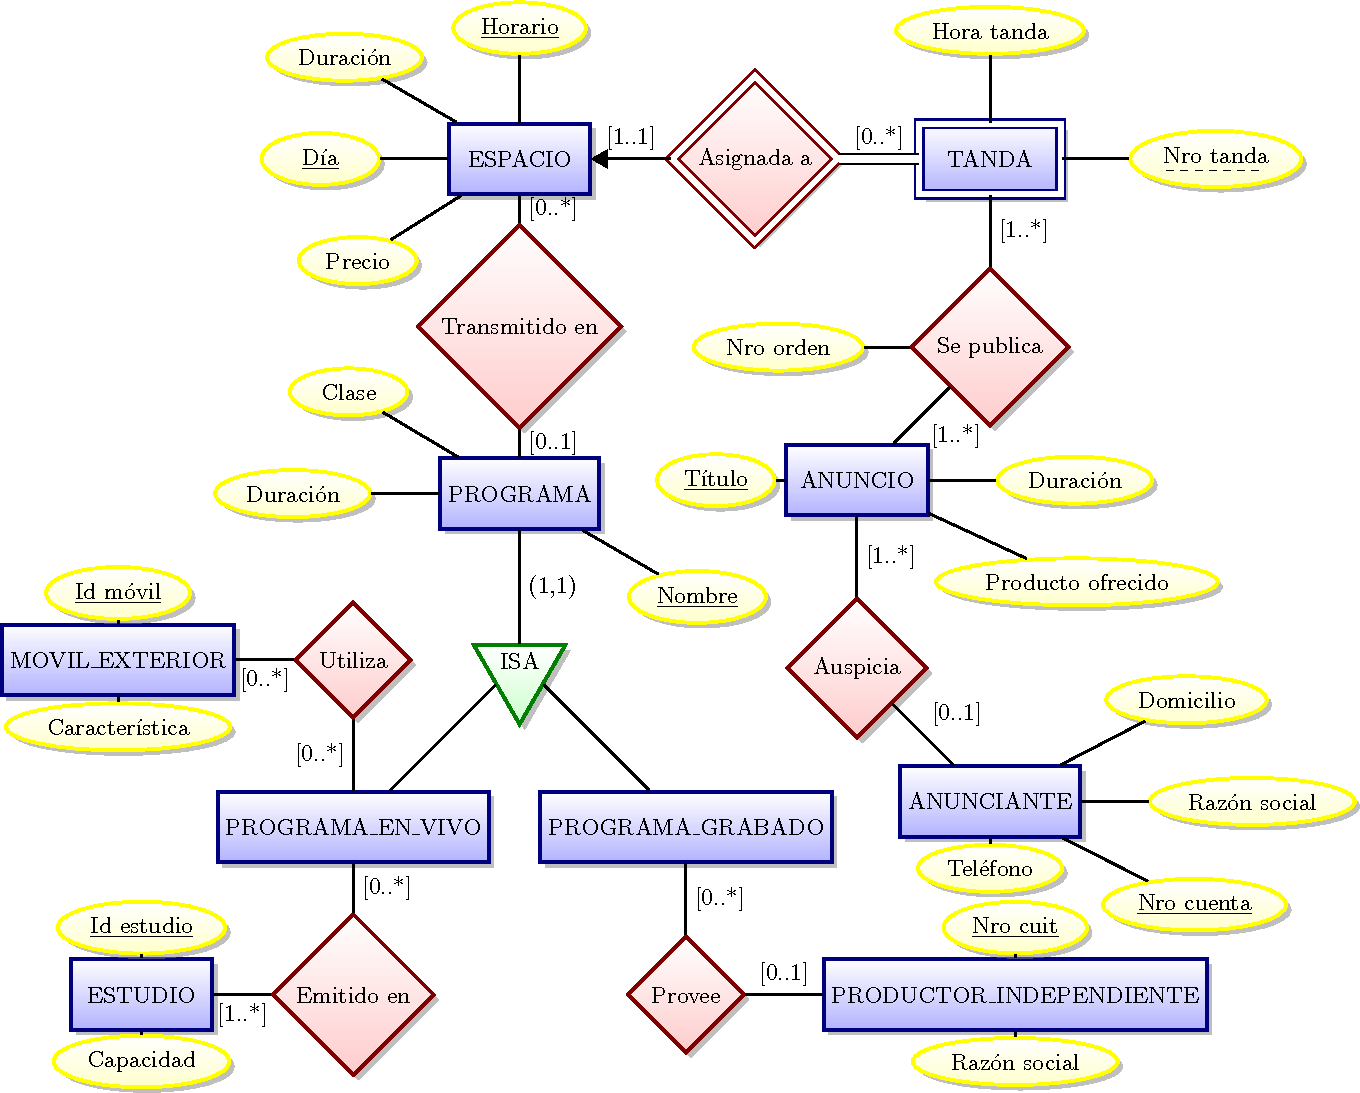
\includegraphics[width=10cm]{ModeloE-R/ModeloE-R.png}
  
  \subsection{Hip\'otesis}
  \begin{enumerate}
    \item Cada m\'ovil de exterior posee un id que lo identifica un\'ivocamente. 
    \item Un programa puede ser en vivo o puede ser grabado.
  \end{enumerate}

\newpage
\section{Transformaci\'on del Modelo E-R a un Modelo Relacional}

%APENDICES
\appendix
\newpage
\section{Enunciado}
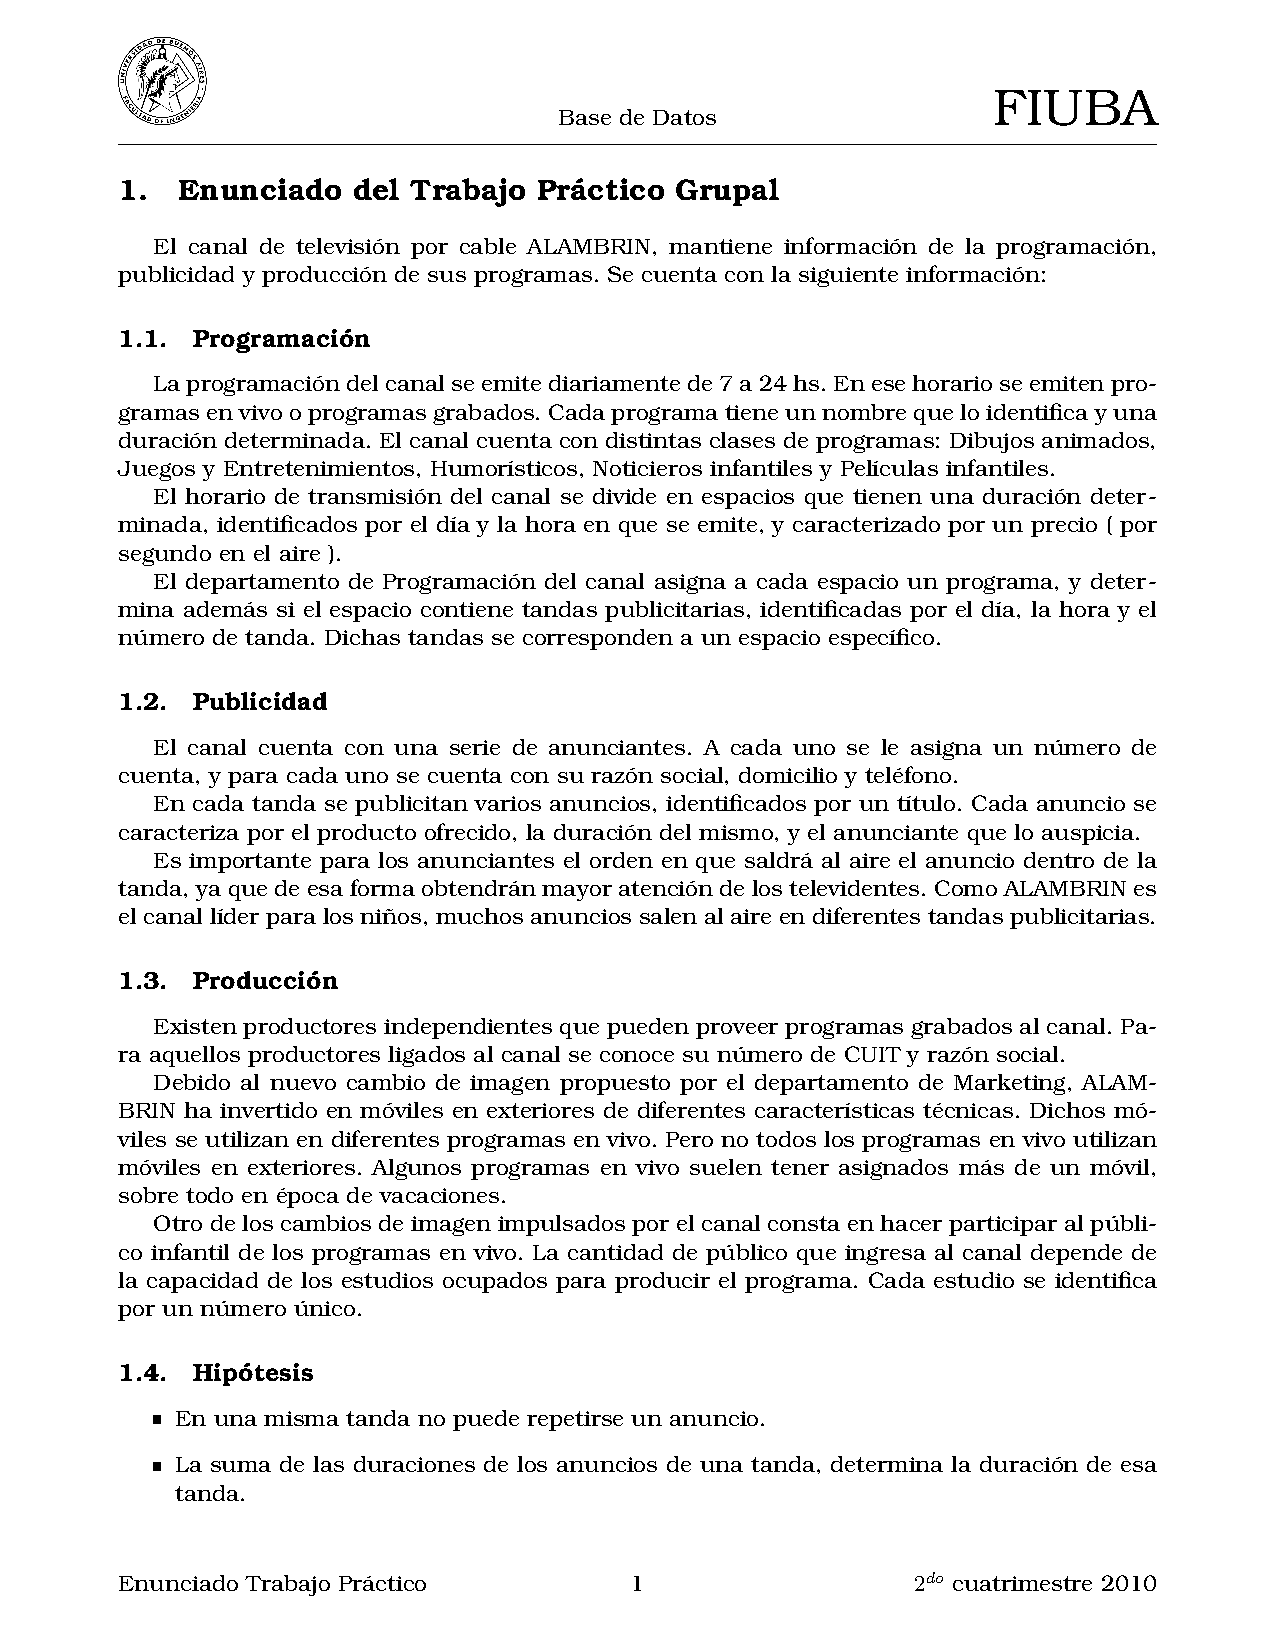
\includepdf[pages=1-2, scale=0.9, pagecommand={\thispagestyle{plain}}]{EnunciadoBD.pdf}

\end{document}
